\chapter{توضیح مختصری بر الگوریتم}\label{ch:alg}

در فصل \ref{ch:rl} در مورد مفاهیم \w{rl} بحث شد. مهمترین مفاهیم عبارتند از:
\begin{multicols}{3}
\begin{enumerate}
	\item \w{env} \item \w{agent} \item \w{env state} \item \w{agent state} \item \w{reward} \item \w{observ} 
\end{enumerate}
\end{multicols}

هدف در این پروژه این بود که یک \w{autocar} با استفاده از الگوریتم های \w{rl} ساخته شود. جزییات تئوری الگوریتم و جزییات فنی پروژه به ترتیب در بخش های 
\ref{ch:rl}
و
\ref{ch:fani}
آورده شده‌اند.
در این بخش به شبیه سازی و جزییات کار و تعریف پارامتر های این پروژه برداخته می‌شود.

\section{معرفی محیط شبیه سازی}

در ابتدا محیط شبیه سازی را معرفی می‌کنیم. جزییات فنی این محیط در \ref{ch:fani} و همچنین نحوه راه‌اندازی آن در بخش \ref{ch:resault|sec:launch} به‌صورت کامل مورد بحث قرار گرفته است. اگر آن محیط را باز کنید محیط مانند شکل 
\ref{fig:obs-1}
باز خواهد شد. این محیط دو آبجکت مهم دارد؛
\begin{alphinline}
	\item ماشین(اتومبیل)
	\item جاده
\end{alphinline}
(شکل \ref{fig:road-car-models}) 



\begin{figure}
	\centering
	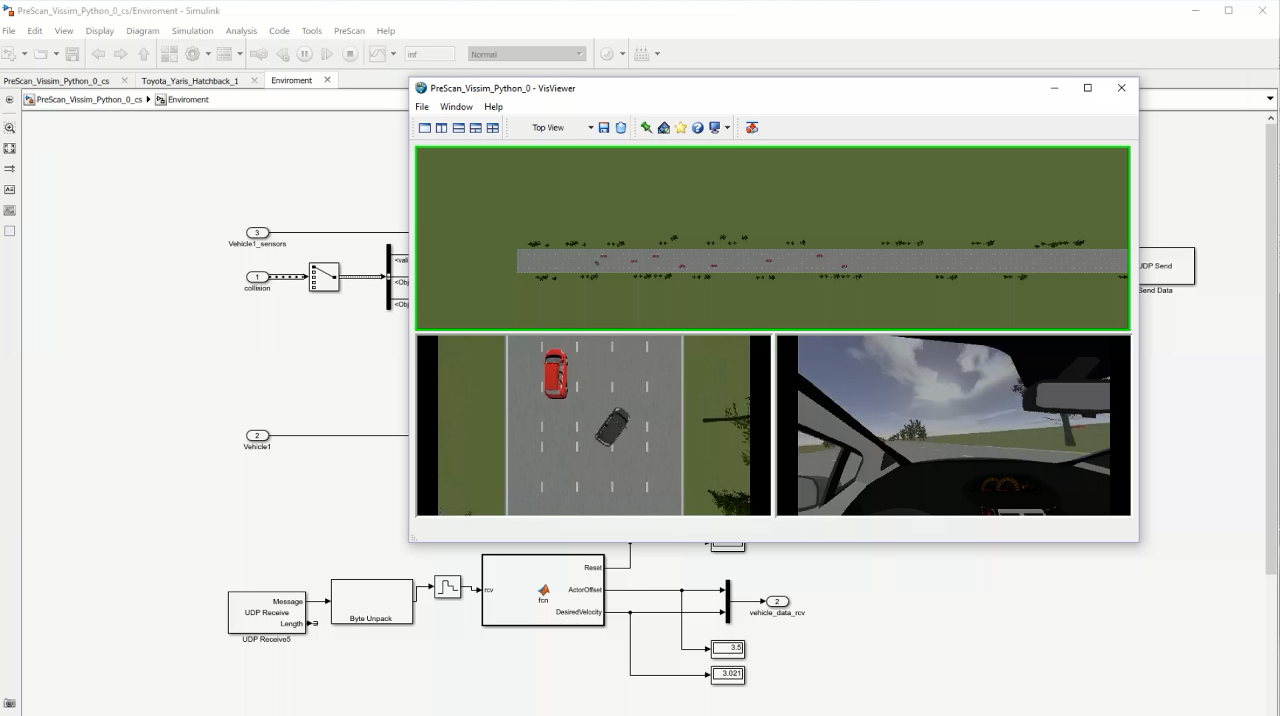
\includegraphics[width=0.7\linewidth]{Figures/OBS/1}
	\caption{محیط شبیه سازی}
	\label{fig:obs-1}
\end{figure}


%HERE
\begin{figure}
	\centering
	\def\localheight{2cm}
	\subfigure[]{%
		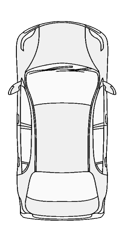
\includegraphics[height=\localheight]{Figures/rzbinary/agent}
		\label{subfig:model-car}
	}
	\hspace*{0.5cm} % space between two figures
	\subfigure[]{%
		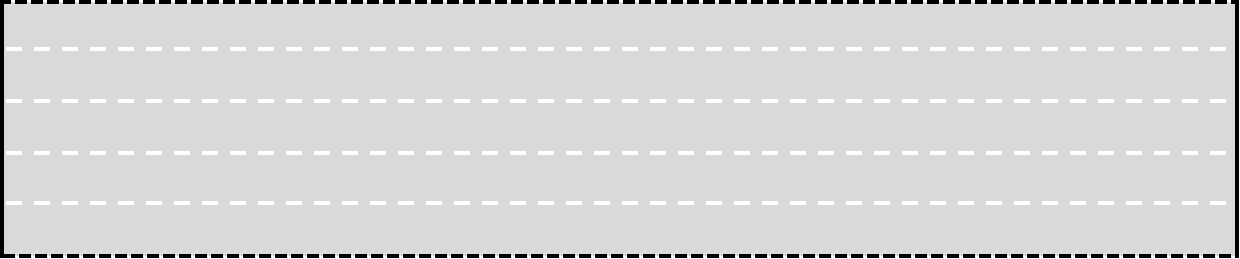
\includegraphics[height=\localheight]{Figures/rzbinary/road}
		\label{subfig:model-road}
	}
	\caption[]{%
	}
	\label{fig:road-car-models}
\end{figure}


چیزی که اهمیت دارد اندازه ها و نحوه تعریف محدوده هاست. شکل \ref{fig:road-car-total} اندازه‌ها و محدوده ها را مشخص کرده است. 
شکل \ref{subfig:road-car-redbox-w} نشان می‌دهد که این محدوده ها کاملا برروی یک دیگر منطبق نیستند. دلیل اصلی این موضوع عدم اهمیت تطبیق دقیق این دو می‌باشد. در بخشی که پشت ماشین قرار دارد این محدوده از $-4$ (کمی بیشتر از اندازه عرض لاین ها) شروع می‌شود. زیرا نیازی نیست بیشتر از این مقدار ماشین مورد بررسی به عقب برود تا متوجه شویم اشتباه در حال رفتن است. درحقیقت این مورد کمک می‌کند تا تعداد \w{step} ها را در هر \w{episode} اشتباه کاهش یابد. بخش های کناری نیز از $-11$ تا $+11$ محدود شده‌اند (بیشتر از عرض خود جاده) تا اگر نوسانی یافت به ماشین این اجازه داده شود تا به مسیر اصلب برگردد. 



\begin{note}
	ماشین در مبدا صفحه قرار دارد. از این رو اعداد منفی نسبت به همین ماشین نیز سنحیده می‌شوند.
\end{note}



\begin{figure}[b!]
	\centering
%	\def\localdata{}
	\subfigure[مشخصات جاده]{%
		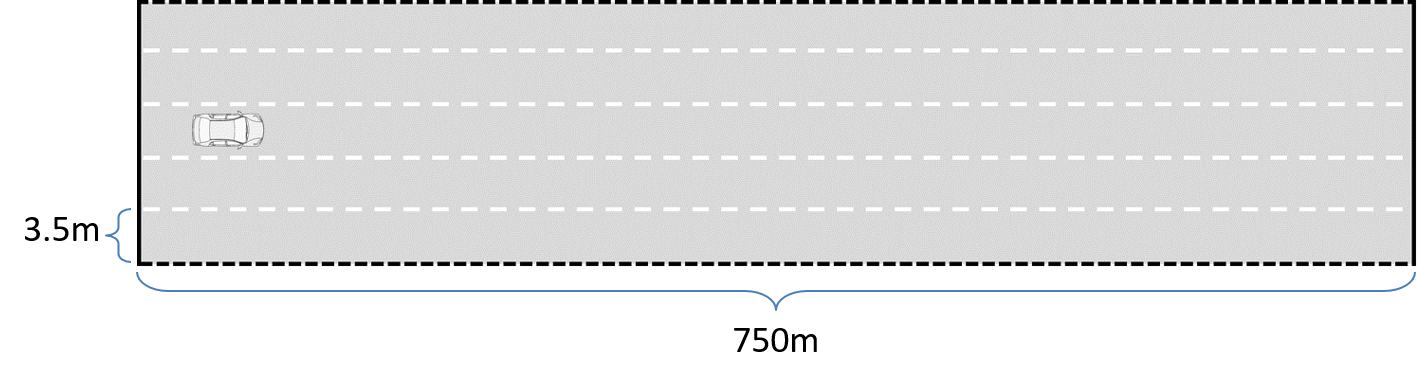
\includegraphics[width=0.7\linewidth]{Figures/rzbinary/road-car-wh}
		\label{subfig:road-car-wh}
	}
	%  	\hspace*{1.5cm} % space between two figures
	\subfigure[محدوده جاده]{%
		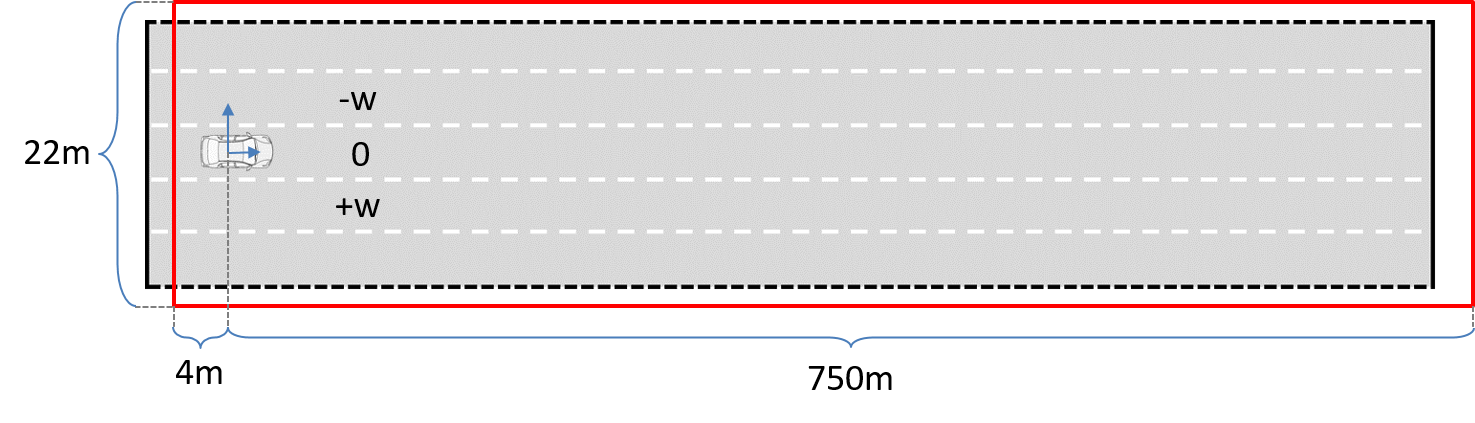
\includegraphics[width=0.7\linewidth]{Figures/rzbinary/road-car-redbox+-w}
		\label{subfig:road-car-redbox-w}
	}
	\caption{
		بررسی دقیق محدوده و مشخصات جاده
	}
	\label{fig:road-car-total}
\end{figure}

3 مقدار \lr{+w} ، \lr{-w} و \lr{0} که در شکل \ref{subfig:road-car-redbox-w} بر روی جاده نوشته شده است در حقیقت مرتبط با بحث فنی ماجرا می‌باشد اما مفهوم آن این است که \w{agent} مورد بررسی می‌تواند این سه لاین را به عنوان \w{action} اختیار کند. در حقیقت می‌توان آن‌ها را به عنوان اسم برای هر لاین در نظر گرفت. در مورد \w{action} بیشتر صحبت خواهد شد.

\begin{note}
	راه‌اندازی این محیط کمی دردسر خواهد داشت از این‌رو نیاز است پیش از راه‌اندازی بخش \ref{ch:resault|sec:launch} به‌طور دقیق مطالعه شود.
\end{note}





\section{معرفی \ws{api} و \ws{alg}}
%\section{تعریف کردن پارامتر های \ws{rl}}
%قبل از بررسی پارامتر های ‌\w{rl} مناسب است که شکل نهایی این الگوریتم همین ابتدا بررسی شود.
%\footnote{منظور از پارامتر های \w{rl} پارامتر هایی مانند تعیین \w{reward} و \w{state} می‌باشد.}
در این پروژه دو الگوریتم \gls{a:dqn} و \gls{a:a2c} بهتر از سایر الگوریتم ها عمل کردند اما در نهایت با توجه به آزمایش‌ها و ملاحظاتی که انجام شد، الگورینم \gls{a:dqn} از لحاظ سرعت همگرایی بهتر از الگوریتم \gls{a:a2c} پاسخ داد. بنابراین صرفا برروی این الگوریتم بحث خواهد شد.




\code[python, label={code:dqn.py}]{dqn-train.py}


این کد بخش \w{train} را نشان می‌دهد. بخش \w{test} در تمامی الگوریتم ها مشابه یک دیگر است و از جایی که مدل تعریف می‌شود (در اینجا خط 18) شروع خواهد شد. 

بخش \w{test} در تمامی الگوریتم ها کد زیر است.

\code{alg-test.py}

از روی چند خط آغازین کد
\hyperref[code:dqn.py]{\gls{a:dqn}}
می‌توان دریافت که این کد با استفاده از \lr{gym}\cite{git/gym} و \lr{stable-baseline}\cite{stable-baselines} نوشته شده است.

بخش مهم بعدی متغیری از جنس دیکشنری به نام \texttt{env\_dict} است. این متغیر برای ساختن متغیر \texttt{env} در دستور 
\lr{\texttt{env = gym.make(**env\_dict)}} 
به‌کار می‌رود.
\RTLfootnote{متغیر \texttt{env} در حقیقت نقش \w{env} را در الگوریتم دارد.}
 توضیح این متغیر و اجزای آن در جدول \ref{tab:env-dict} آمده است.
 
\begin{table}\tableset{
\begin{tabular}{|C{0.25\linewidth}|p{0.7\linewidth}|}
	\hline\rowcolor{lightgray}
	متغیر & توضیحات
	\\\hline\hline
	\texttt{id} & در این پروژه این متغیر دو حالت بیشتر ندارد که هردو از جنس رشته هستند. اگر این کد با استفاده از \w{matlabengine} استفاده شود، \lr{\texttt{'prescan-v0'}} 
	خواهد بود و اگر از \w{matlabengine} استفاده نشده باشد مقدار آن 
	\lr{\texttt{'prescan-without-matlabengine-v0'}} 
	خواهد بود. 
	
	این متغیر مقدار پیش‌فرض ندارد.
	 \\\hline
	\texttt{verbose} & این متغیر که از جنس بولین می‌باشد، در صورتی که یک باشد اطلاعات جامعی را در هر \w{step} 
	را چاپ می‌کند. علاوه برآن اطلاعات آماری \w{reward}های بدست‌آمده در پایان هر \w{episode} را نیز چاپ می‌کند. به‌طور کلی اجازه گزارش دادن و ندادن اطلاعات درونی الگوریتم توسط این متغیر کنترل می‌شود.
	 \\\hline
	\texttt{host} & این متغیر برای اتصال شبکه بین دو کامپیوتر به کار می‌رود و در حقیقت \lr{IP} کامپیوتری است که ویندوز بر روی آن نصب است. مقدار پیش‌فرض این متغیر \texttt{'localhost'} می‌باشد. \\\hline
	\texttt{delay} & همان‌طور که مشخص است این متغیر مقدار تاخیر را مشخص میکنم و مورد کاربرد آن لحظه ای است که \texttt{action} در تابع \texttt{step} فرستاده شده است و پس از گذشت مقداری تاخیر برحسب ثانیه سعی در دریافت اطلاعاتی مانند \w{obs} بعدی و محاسبه \w{reward} و ... داریم. مقدار پیش‌فرض این متغیر نیز صفر است. \\\hline
	\texttt{nget} & این متغیر نیز به نوعی متفاوت تاخیر را شکل می‌دهد. این متغیر از نوع عدد صحیح می‌باشد و هنگامی که مقدار آن 150 است یعنی محل تاخیر، 150 بار داده‌ها را دریافت می‌کند و مقدار آن‌ها را می‌خواند. در حالت عادی تا پایان 150‌اُمین دریافت هیچ کاری نمی‌کند مگر این که مقدار \texttt{done} برابر یک شود؛ در این صورت حلقه را متوقف کرده و باقی عملیات را انجام می‌دهد. 
	مقدار پیش‌فرض این متغیر یک می‌باشد.
	\\\hline
	\texttt{experimant\_name} & این متغیر مربوط به تنظیمات \w{matlabengine} می‌باشد و به صورت عادی نیازی به تغییر مقدار پیش‌فرض آن نیست.\\\hline
	\texttt{close\_window} & این پارامتر درصورتی قابل اجراست که کد پایتون و نرم‌افزار \w{prescan} هردو بر روی یک کامپیوتر باشند و وظیفه آن این است که محیط گرافیکی را پس از اجرا شدن کد می‌بندد و مقدار پیش فرض آن صفر می‌باشد. \\\hline
\end{tabular}}
\caption{بررسی پارامتر های موجود در \texttt{env\_dict}}
\label{tab:env-dict}
\end{table}

همان‌طور که در جدول \ref{tab:env-dict} توضیح داده‌شده‌است؛ دو متغیر \texttt{nget} و  \texttt{delay} هر دو از جنس تاخیر می‌باشند. محل تاخیر در تابع \texttt{step} می‌باشد. کد زیر محل تاخیر را نشان می‌دهد.

\begin{latin}
\begin{lstlisting}
def step(self, action):	
	self.send(action)
	# -------- BEGIN DELAY --------
	if self.delay > 0 :
		sleep(self.delay)
	for _ in range(self.nget):
		self.render_()
		if self.done:
			break
	# --------- END DELAY -‌--------
	observation = self._next_observation()
	reward = self.calc_reward()
	done = self.done
	info = {'Collision':self.collision ,'Position':self.agent['data']['Position']}
\end{lstlisting}
\end{latin}

این کد که در حقیقت هسته اصلی
\RTLfootnote{این کد از آن جهت که کاملا با تابع اصلی برابر نمی‌باشد، واژه "هسته اصلی" برای آن در نظر گرفته شده است. تفاوت آن با کد اصلی برخی عملیات است که مرتبط با چاپ شدن اصلاعات در حال اجرا می‌باشد که به مقدار \texttt{verbose} مرتبط می‌شود.}
 تابع \lr{step} می‌باشد. در بین محدوده مشخص شده، تاخیر صورت می‌گیرد. همان طور که مشخص است این تاخیر بین فرستادن \w{action} و محاسبه پارامتر‌هایی مانند \w{reward} و \w{obs}(\w{state})
می‌باشد. 
\begin{note}
	علت اصلی وجود تاخیر، مهلت دادن به \w{agent} برای انجام \w{action} است.
\end{note}

دو متغیر \texttt{nget} و \texttt{delay} هردو وظیفه ایجاد تاخیر دارند که نحوه ایجاد این تاخیر با یک‌دیگر کاملا متفاوت است. همچنین این امکان نیز وجود دارد به صورت ترکیبی نیز این تاخیر را ایجاد کرد. هر کدام از این روش‌ها مزایا و معایب خاص خود را دارند.

مزیت مهم استفاده از \texttt{nget} این است که به‌صورت مداوم در‌حال دریافت اطلاعات از محیط شبیه‌سازی است. بنابراین در صورت رخ دادن اتفاق خاصی مانند تصادف کردن و یا از مسیر خارج شدن می‌تواند آن‌را به موقع تشخیص دهد و تصمیمات لازم را انجام دهد.
در صورتی که در زمانی که تاخیر ناشی از \texttt{delay} است، عملا در آن مدت ارتباط با محیط شبیه سازی قطع شده است و ممکن است رخ دادن موارد گفته شده یا بسیار دیر متوجه شود و یا اصلا متوجه نشود. 

به‌طور مثال درصورتی که دو ماشین با یکدیگر تصادف داشته باشند؛ اگر این رخداد سریعا تشخیص داده نشود، در این صورت احتمال دارد این دو ماشین از روی یک دیگر عبور کنند! و پس از عبور کردن این اطلاعات دریافت شود و برخوردی تشخیص داده نشود. از آن‌جا که برخورد بیشترین میزان تاثیر در \w{reward} دارد؛ بنابراین، این اتفاق تاثیرات خیلی مخربی می‌تواند بر الگوریتم بگذارد.

عیب اصلی روش \texttt{nget} نیز این است که یک مقدار مشخص ندارد و به پارامتر هایی از جمله سرعت شبکه نیز وابسته است. بنابراین اگر از یک شبکه به شبکه دیگر منتقل شود می‌تواند مقدار کاملا متفاوتی به خود گیرد که شاید مطلوب نباشد. اما به راحتی با عوض کردن مقدار این متغیر در لایه \w{alg} می‌توان این مشکل را حل کرد. بنابراین توصیه می‌شود از این متغیر استفاده شود.



به کد 
\hyperref[code:dqn.py]{\gls{a:dqn}}
برگردیم.
خط 18 این کد مدل را می‌سازد. چیزی که اهمیت دارد این است که پارامتر $\gamma$ چه مقداری انتخاب شود. در نسخه نهایی این مقدار روی $0.8$ تنظیم شده است. در مورد این متغیر در بخش \ref{ch:rl} و در مراجع \cite{Sutton1998} و  \cite{uclRL} بحث شده‌است.
در ابتدا این متغیر مقدار پیش‌فرض $0.99$ را داشت. پس از بررسی‌های انجام شده این مقدار به $0.8$ کاهش یافت.

\section{تعریف کردن پارامتر های \ws{rl}}
منظور از پارامتر‌های \w{rl} از متغیر‌های \w{action} و \w{state} و \w{reward} و ... تا تعریف برخی توابع می‌باشد. 
ابتدا کلیات توابع را بررسی کنیم و سپس وارد جزییات آن پارامتر ها می‌شویم.

توابع استفاده شده به دو دسته تقسیم می‌شوند.
\begin{alphinline}
	\item توابع اصلی 
	\item  توابع فرعی یا کمکی
\end{alphinline}.

توابع اصلی آن دسته از توابعی هستند که مختص به کتاب‌خانه \texttt{gym} هستند و قرار دادن آن ها به شکل صحیح آن، اجباری است. توابع کمکی آن دسته از توابعی هستند که در این توابع نقش های مشخصی را ایفا کردند ولی استفاده کردن از آن ها اجباری نداشته است. 

\begin{note}
	در صورت لزوم کاربر می‌تواند توابع فرعی را تغییر دهد تا خروجی مطلوب خود را حاصل کند اما در لایه الگوریتم صرفا از توابع اصلی استفاده می‌شود. زیرا هدف هم که استاندارد سازی کد می‌باشد با این موضوع سازگار است.
\end{note}



\begin{table}\tableset{
\begin{tabular}{|C{0.2\linewidth}|p{0.75\linewidth}|}
	\hline\rowcolor{lightgray}
	نام تابع & توضیحات
	\\\hline\hline
	\texttt{\_\_init\_\_} &  این تابع علاوه بر تنظیم کردن برخی پارامترهای مرتبط به کلاس، اتصال کد پایتون به نرم افزار متلب را نیز برعهده دارد.  
	همچنین تعیین \w{obsspace} و  \w{actionspace} نیز بر‌عهده این بخش می‌باشد.
	\\\hline
	\texttt{step} &  این تابع همان \w{step} است که در بخش 
	\ref{ch:rl} مطرح شد. محل اصلی اجرای این تابع در داخل یک حلقه متناهی می‌باشد. این تابع \texttt{action} را به صورت ورودی می‌گیرد و متغیر‌هایی مانند \texttt{observation} ، \texttt{reward} ، \texttt{done} و \texttt{info} را خروجی می‌دهد. در مورد نحوه محاسبه این خروجی ها صحبت خواهد شد.
	  \\\hline
	\texttt{reset} &  این تابع \texttt{env} ،را ریست می‌کند و به عنوان خروجی \w{state} اولیه را بر‌می‌گرداند. موارد استفاده از این تابع معمولا در اول کد و در آخر هر \w{episode} می‌باشد. آخر هر \w{episode} هنگامی فرا می‌رسد که متغیر \texttt{done} که یکی از خروجی‌های تابع \texttt{step} است، یک شود. \\\hline
	\texttt{render} &  این تابع به صورت معمول کارهای گرافیکی را برعهده دارد. اما از آنجایی که عمل در پس زمینه طرح وجود دارد، پس کار اصلی آن گرفتن داده‌ها و منظم کردن آن‌ها می‌باشد. برای این کار از یک تابع کمکی به نام \texttt{render\_} استفاده می‌کند.  \\\hline
\end{tabular}}
\caption{راهنمای توابع اصلی \ws{api}}
\label{tab:gym-alg-env}
\end{table}


جدول \ref{tab:gym-alg-env}، توابع اصلی را نشان می‌دهد و جدول \ref{tab:aux-alg-env} نیز توابع کمکی را نشان می‌دهد. همچنین لازم به ذکر است که 
\hyperref[code:standard-test]{کد تست استاندارد}
 این پروژه در به صورت زیر است:

\code[python,label={code:standard-test}]{standard-test.py}




\begin{table}[h!]\tableset{
\begin{tabular}{|C{0.25\linewidth}|C{0.16\linewidth}|p{0.54\linewidth}|}
\hline\rowcolor{lightgray}
نام تابع
&
محل استفاده
&
توضیحات
\\\hline\hline
\texttt{make}
&
\texttt{\_\_init\_\_}
&
این تابع لایه ای را ایجاد می‌کند که هرگونه ارتباط با محیط شبیه‌سازی به آن لایه مرتبط می‌شود.
\\\hline
\texttt{render\_}
&
\texttt{render} و 
\texttt{step} و 
\texttt{reset}
&
این تابع وظیفه دریافت اطلاعات از محیط شبیه سازی و استخراج داده‌های مفید از آن است.
\\\hline
\texttt{send}
&
\texttt{step}
&
این تابع برای فرستادن \w{action} به محیط شبیه سازی استفاده می‌شود.
\\\hline
\texttt{calc\_reward}
&
\texttt{step}
&
این تابع \w{reward} را محاسبه می‌کند.
\\\hline
\texttt{\_next\_observation}
&
\texttt{reset} و
\texttt{step}
&
این تابع \w{state} بعدی \w{agent} را محاسبه می‌کند.
\\\hline
\texttt{action\_translate}
&
\texttt{send}
&
این تابع مانند یک \ws{joystick} در تابع \texttt{send} \w{action} را تفسیر می‌کند و دستورات کنترلی قابل اجرا برای محیط شبیه‌سازی ایجاد می‌کند.
\\\hline
\end{tabular}}
\caption{راهنمای توابع کمکی \ws{api}}
\label{tab:aux-alg-env}
\end{table}

\begin{note}
	این کد صرفا صحت عملکرد و نحوه استفاده از \w{api} را نشان می‌دهد و شامل هیچ گونه الگوریتمی نمی‌باشد.
\end{note}

\subsection{معرفی برخی توابع \ws{api}}

\subsubsection{بررسی تابع \textbf{\texttt{\_\_init\_\_} :}}
این تابع سه وظیفه مهم دارد. 
\begin{alphabetlist}
	\item 
	بخشی از وظایف آن، وظایف مشخص آن در کد پایتون است.
	\item 
	ست کردن برخی پارامتر های مهم که در جدول \ref{tab:env-dict} نیز آمده‌اند.
	\item 
	این تابع  \w{obsspace} و \w{actionspace} را مشخص می‌کند.
\end{alphabetlist}
اطلاعات \w{obsspace} و \w{actionspace} در جدول \ref{tab:spaces-alg} آمده‌است.

\begin{table}\tableset{
\begin{tabular}{|c|c|C{0.35\linewidth}|c|}
	\hline\rowcolor{lightgray}
	نام متغیر& مفهوم& جنس متغیر& توضیحات\\\hline
	\hline
	\texttt{action\_space} & \w{actionspace} & \lr{\texttt{spaces.Discrete(6)}} & عدد صحیح 6\\\hline
	\texttt{observation\_space} & \w{obsspace} & \lr{\texttt{spaces.Box(shape=(1,38), dtype=np.float16)}} & ماتریس 
	$1\!\times\!38$تایی \\\hline
\end{tabular}}
\caption{تعریف \ws{obsspace} و  \ws{actionspace} در پروژه}
\label{tab:spaces-alg}
\end{table}



\subsubsection{بررسی تابع \textbf{\texttt{action\_translation} :}}
این کد دقیقا پیاده سازی یک \w{joystick} می‌باشد. شکل \ref{fig:minipage-joystick} اطلاعات کامل این موضوع به همراه تفسیر آن ها دارد. 

از آنجایی که در این پروژه \w{actionspace} طبق جدول \ref{tab:spaces-alg} مقدار عدد صحیح 6 را دارد و این به آن معناست که 6 حالت گسسته بین صفر تا 5 برای \w{action} وجود دارد همچنین نشان می‌دهد که جنس \texttt{action} عدد صحیح \texttt{int} است. بنابراین، می‌بایست که آن را تفسیر کرد. وظیف اصلی این تابع نیز تفسیر مقدار مختلفی است که \texttt{action} می‌تواند بگیرد، می‌باشد.
 
%self.action_space = spaces.Discrete(6)
%self.observation_space = spaces.Box(low=0, high=255, shape= (1, 38), dtype=np.float16)





%\newlinef
\begin{figure}
\begin{minipage}{4.8cm}
\centering
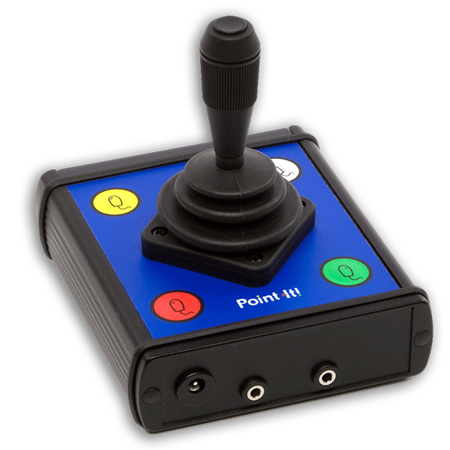
\includegraphics[width=4.8cm]{Figures/joystick}
\label{fig:joystick}
\\[2em]
\tableset[1.5]{\begin{tabular}{c||c}
	شماره & وظیفه
	\\\hline\hline
	0 & رفتن به لاین \texttt{-w}\\
	1 & رفتن به لاین \texttt{0}\\
	2 & رفتن به لاین \texttt{+w}\\
	3 & زیاد کردن سرعت \\
	4 & کم کردن سرعت \\
	5 & بدون تغییر \\
\end{tabular}}
\end{minipage}
\hspace*{0.5cm}
\begin{minipage}{10cm}
\code[python,label={code:joystick}]{action-translation.py}
\end{minipage}
\caption{بررسی تابع \texttt{action\_translate}}
\label{fig:minipage-joystick}
\end{figure}

\begin{note}
	دستور کنترلی اصلی یک بردار دوتایی است (خط  18 کد شکل \ref{fig:minipage-joystick}) که مقدار اولی آن لاین را نشان می‌دهد و مقدار دوم آن سرعتی می‌باشد که انتظار داریم که \w{agent}، سرعت خود را به آن برساند. 
\end{note}
\begin{note}
	اگر دقت کنید در کد مذکور دو مقدار کنونی و قدیمی تر \texttt{action} نگه‌داری شده است.
\end{note}
\begin{note}
	همچنین دقت شود که در این کد، مقدار سرعت، همان مقدار حقیقی سرعت است که از محیط شبیه‌سازی می‌آید. و مقداری که در بردار \texttt{\_\_action\_\_} قرار می‌گیرد مقدار کنترلی سرعت است که با یک‌دیگر تفاوت دارند.
\end{note}


%\begin{latin}
%\begin{lstlisting}
%def action_velocity(vel,increase):
%	if increase:
%		return vel+5
%	else:
%		if vel < 5:
%			return vel/2
%		else:
%			return vel - 2
%\end{lstlisting}
%\end{latin}

نکته دیگری که حایز اهمیت است این است که هنگامی که گزینه 3 و یا 4 انتخاب می‌شوند، سیاستی برای افزایش و کاهش سرعت اتخاذ شده است. این سیاست در قالب یک تابع در تصاویر شکل \ref{fig:action-velocity-total} ظاهر شده است. همانطور که کد \ref{subfig:action-velocity-code} و نمودار متناظر آن در شکل \ref{subfig:action-velocity-double} نشان می‌دهد، سیاست های مختلفی برای زیاد کردن و کم کردن سرعت اتخاظ شده است. 

برای زیاد کردن سرعت، سرعت واقعی که از محیط شبیه سازی دریافت شده است با 5 واحد جمع می‌شود. بنابراین انتظار داریم سرعت پس از سه بار افزایش به 15 برسد (شکل \ref{subfig:action-velocity-inc}، نمودار قرمز) اما این اتفاق نمی‌افتد. زیرا این افزایش سرعت، کار زمان‌بری است و 
نیاز به حوصله دارد که اگر حوصله و تحمل و به عبارت دیگر تاخیر را از یه حدی بالاتر ببریم عملا در کنترل \w{agent} به مشکل خواهیم رسید. 

همچنین مورد مشابه آن چه که گفته شد، در شکل \ref{subfig:action-velocity-dec} نیز برقرار است. نقاطی که رنگشان قرمز است نمودار ایدآلی مفروض خواهند بود که معادل تاخیر کم سیستم جهت اعمال سرعت نهایی است. و نمودار دیگر معادل رخدادی است که $30\%$ به آن عمل شده است و $70\%$ تحت تاثیر مقدار قبلی خواهد بود و به این صورت یک میانگین وزن‌دار گرفته شده‌است.

\begin{figure}
\centering
\subfigure[کد اصلی روند افزایشی و یا کاهشی سرعت]{%
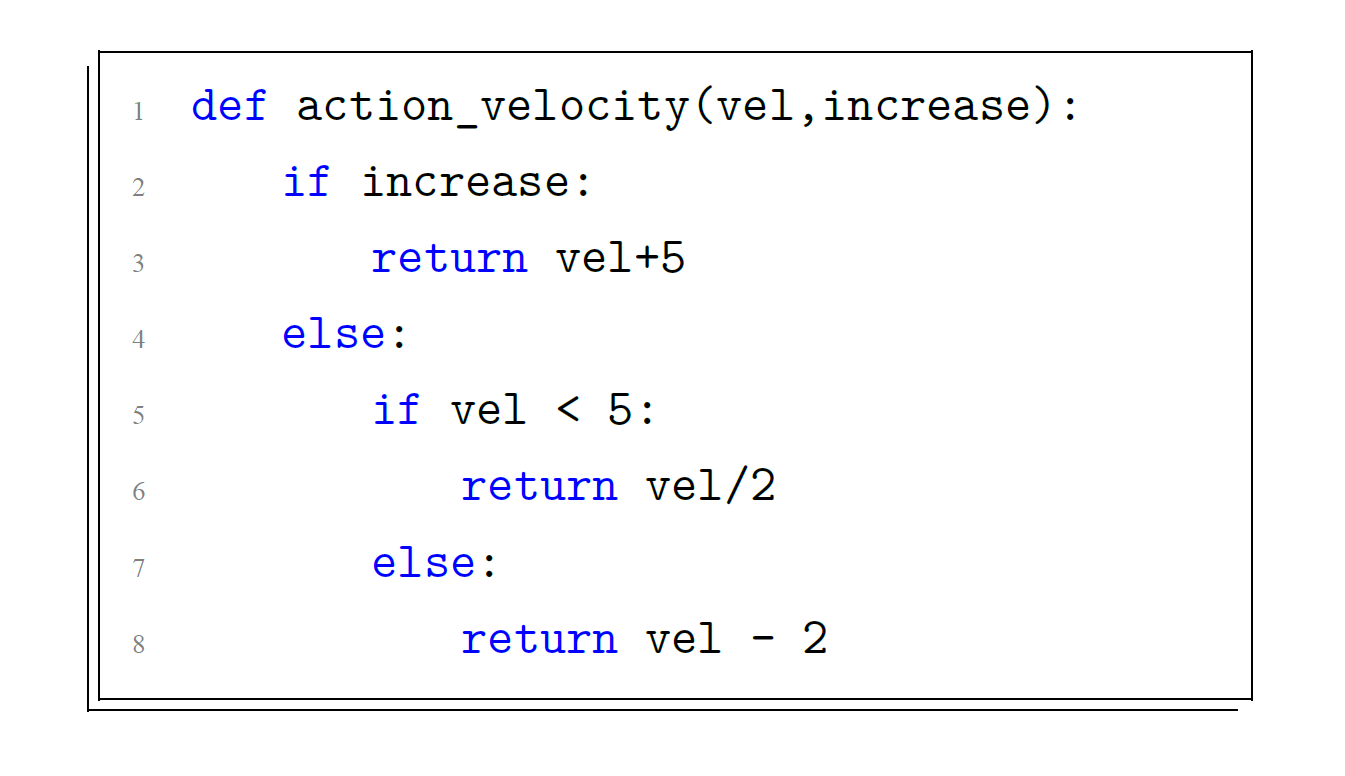
\includegraphics[height=3.7cm]{Figures/code/action-velocity-code2}
\label{subfig:action-velocity-code}
}
\hspace*{0.5cm} % space between two figures
\subfigure[شکل کلی نمودار افزایش سرعت]{%
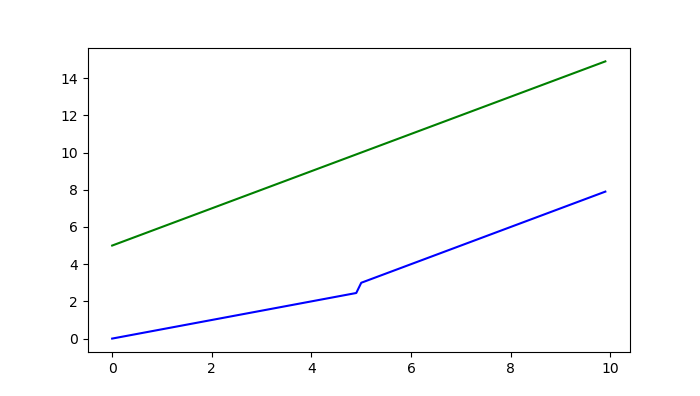
\includegraphics[height=4cm]{Figures/code/action-velocity-double}
\label{subfig:action-velocity-double}
}
%	\hspace*{0.5cm} % space between two figures
\subfigure[حرکت در جهت افزایش سرعت با شروع از صفر]{%
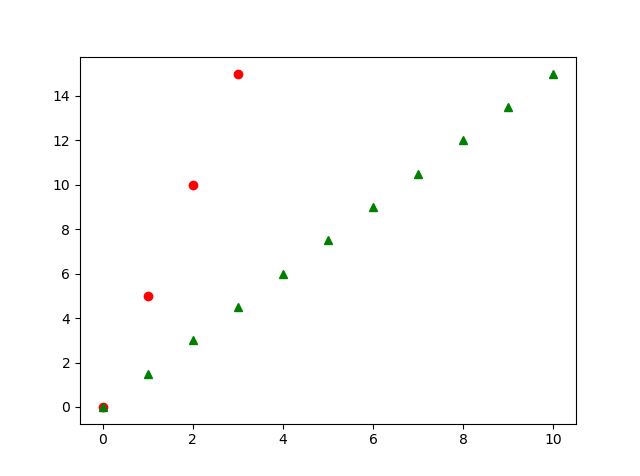
\includegraphics[height=5cm]{Figures/code/action-velocity-inc}
\label{subfig:action-velocity-inc}
}
\subfigure[حرکت در جهت کاهش سرعت با شروع از 10]{%
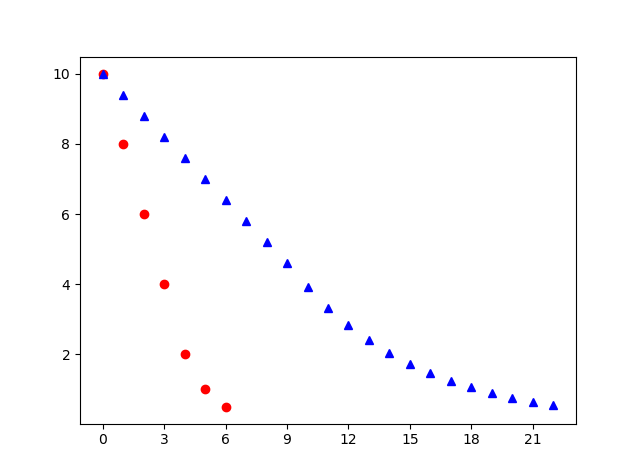
\includegraphics[height=5cm]{Figures/code/action-velocity-dec}
\label{subfig:action-velocity-dec}
}
%	\hspace*{0.5cm} % space between two figures
\caption{%
	بررسی دقیق تابع افزایش دهنده و کاهنده سرعت ماشین
}
\label{fig:action-velocity-total}
\end{figure}

مشاهده می‌شود که مسیری که به واقعیت نزدیک‌تر است آرامتر از مسیر مدنظر است. همچنین تفاوت تغییر روند کاهشی سرعت های کمتر از 5 واحد، این است که هیچ گاه منفی نشود ولی به صورت نمایی کاهش یابد و نزدیک صفر شود.

 تفاوت دیگر آن است که به هنگام افزایش مقدار 5 واحد به سرعت افزوده می‌شود و در هنگام کاهش مقدار دو واحد (برای سرعت های بالای 5 واحد) از آن کسر می‌شود. این تفاوت در مقایسه فاصله نقاط بین دو نمودار شکل‌های \ref{subfig:action-velocity-inc} و  \ref{subfig:action-velocity-dec} نیز ظاهر شده است. علت اصلی این تفاوت در بررسی \texttt{calc\_reward} خود را نشان می‌دهد. اما پیشتر در نظر داشته باشید که یک سیاست چهت‌دار و تشویقی جهت قرار گرفتن سریع‌تر در مسیر درست می‌باشد.
 
\subsubsection{بررسی تابع \textbf{\texttt{step} :}}

کد این تابع را پیش تر بررسی شد. جایگاه این تابع داخل 
\hyperref[code:standard-test]{کد تست استاندارد}
در داخل یک حلقه است هنگامی که حلقه تمام شود به اصلاح یک \w{episode} تمام شده‌است. دلیل تمام شدن حلقه یا رسیدن به سقف تعداد \w{step} در هر \w{episode} است و یا یک شدن مقدار \texttt{done}. این مقدار یکی از خروجی هایی است که این متغیر می‌تواند اختیار کند.
 
این تابع مقدار \w{action} را می‌گیرد. سپس آن را برای محیط شبیه سازی می‌فرستد. در کد زیر این کار توسط تابع \texttt{send} انجام می‌پذیرد. در تابع \texttt{send} ابتدا با استفاده از تابع \texttt{action\_translate} به صورت دستور کنترلی در خواهد آمد و پس از این تبدیل برای محیط شبیه سازی ارسال می‌شود.

پس از مقداری تاخیر، متغیر های \texttt{observation} و  \texttt{reward} که به ترتیب \w{obs} و \w{reward} می‌باشند، محاسبه می‌شود. در کنار این دو خروجی، خروجی‌های دیگری وجود دارند. \texttt{done} که از محیط شبیه سازی می‌آید و نشان می‌دهد که \w{episode} تمام شده‌است. متغیر \texttt{info} متغیری است که اطلاعات اضافه‌ای را خروجی می‌دهد که در دیباگ کردن مفید خواهد بود. این اطلاعات اضافی در این پروژه، اطلاعات برخورد و اطلاعات موقعیت \w{agent} انتخاب شده اند.

\begin{note}
	نحوه محاسبه \texttt{done} وظیفه محیط شبیه‌سازی می‌باشد. منطق محاسبه آن در شکل \ref{fig:done-step-logical} آمده است.  نبابراین اطلاعات دو حالت وجود دارد که موجب تمام شدن یک \w{episode} و به‌طور معادل یک شدن \texttt{done} می‌شود: 
	\begin{alphabetlist}
		\item خارج شدن از محدوده جاده
		\RTLfootnote{منظور از محدوده جاده، محدوده‌ای است که در شکل \ref{subfig:road-car-redbox-w} مشخص شده است.}
		\item تصادف کردن با ماشین دیگر
	\end{alphabetlist}
\end{note}
\begin{note}
	مدار منطقی شکل \ref{fig:done-step-logical} علاوه بر محاسبه متغیر \texttt{done}، در مورد نحوه ریست شدن محیط نیز تصمیم‌گیری می‌کند که مرتبط به بخش فنی است و در این لایه بررسی ‌نمی‌شود.
\end{note}

\begin{figure}
	\centering
	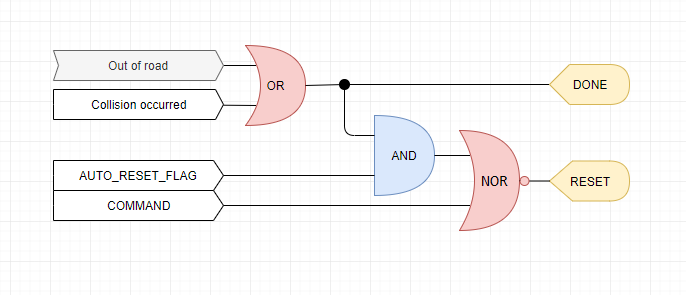
\includegraphics[width=0.7\linewidth]{Figures/done-reset-logical}
	\caption{منطق محاسبه \texttt{done} در محیط شبیه‌سازی}
	\label{fig:done-step-logical}
\end{figure}




کد این تابع در زیر آمده است. دو تابع \texttt{\_next\_observation} و \texttt{calc\_reward} به ترتیب \w{obs} و \w{reward} را محاسبه می‌کنند که به صورت جداگانه بررسی خواهند شد.

\begin{latin}
\begin{lstlisting}
def step(self, action):	
	self.send(action)
	# -------- BEGIN DELAY --------
	if self.delay > 0 :
		sleep(self.delay)
	for _ in range(self.nget):
		self.render_()
		if self.done:
			break
	# --------- END DELAY -‌--------
	observation = self._next_observation()
	reward = self.calc_reward()
	done = self.done
	info = {'Collision':self.collision ,'Position':self.agent['data']['Position']}
\end{lstlisting}
\end{latin}

\subsection{بررسی تابع \textbf{\texttt{\_next\_observation} :}}
این تابع مشخص می‌کند که چه چیزی به عنوان \w{obs} اعلام شود. همان‌طور که در جدول \ref{tab:spaces-alg} آمده است، خروجی نهایی این تابع دارای ابعاد $1\!\times\!38$ می‌باشد. شکل \ref{fig:minipage-next-obs} این روند را به‌طور کامل نشان ‌می‌دهد.

بنابراین \w{obs} یک بردار 38 تایی است که 36 داده اول آن بر اساس زاویه و اندازه محاسبه شده است و 2 داده دیگر آن مقدار $y$ و مقدار سرعت($v$) می‌باشد.

\begin{figure}
\begin{minipage}{0.3\linewidth}
\centering
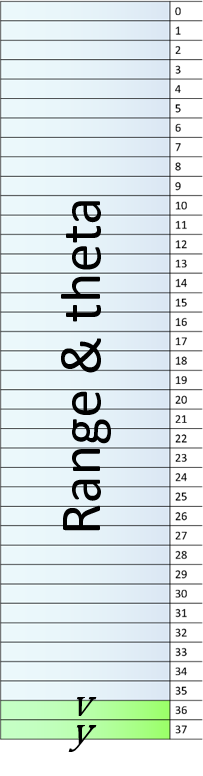
\includegraphics[width=0.7\linewidth]{Figures/rzbinary/observation-reward2-note}	
\end{minipage}
\begin{minipage}{0.7\linewidth}
\code{-next-observation.py}
\end{minipage}
\caption{نحوه تعریف \ws{obs}}
\label{fig:minipage-next-obs}
\end{figure}


بر روی ماشین یک سنسور وجود دارد که دو بردار 10 تایی شامل فاصله و زاویه از 10 ماشین کنار خود را می‌دهد. به این ترتیب برای تعریف \w{obs} فضای اطراف ماشین به 36 قسمت افراز شد به طوری که هر افراز آن یک محدوده به زاویه 10 درجه را شامل می شود. 
شکل \ref{fig:agent-degree-total} طرز تعریف و مقدار دهی این بردار 36 تایی را نشان می‌دهد.
اگر در آن افراز ماشینی قرار نگرفت مقدار آن صفر است و در غیر این صورت فاصله آن با نزدیک‌ترین ماشین خواهد بود.

\begin{figure}
	\centering
	\subfigure[]{
		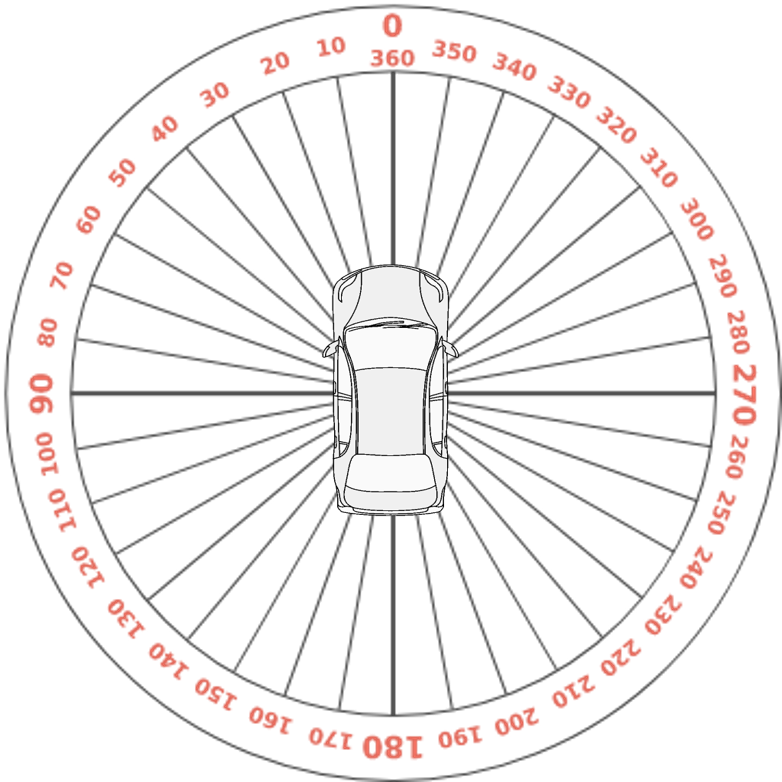
\includegraphics[width=0.4\linewidth]{Figures/rzbinary/agent-degree}
		\label{subfig:agent-degree}	
	}
	\hspace*{0.05\linewidth}
	\subfigure[]{
		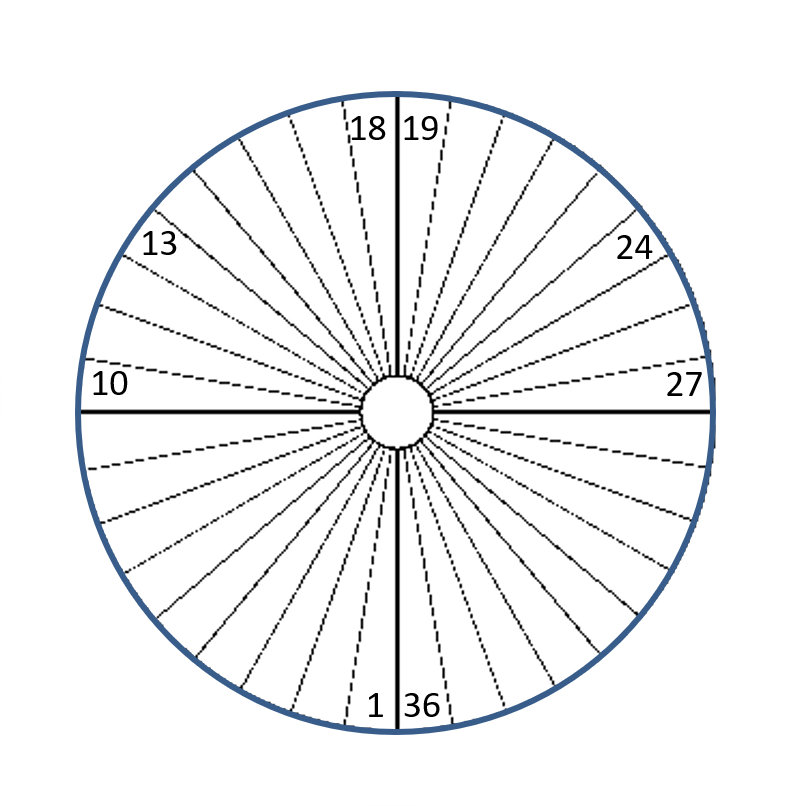
\includegraphics[width=0.39\linewidth]{Figures/rzbinary/circle-number}
		\label{subfig:circle-number}
	}
	\caption[افراز محیط اطراف ماشین برحسب زاویه]{افراز محیط اطراف ماشین برحسب زاویه و تعریف نحوه قرار دادن آن در ماتریس مشاهده }
	\label{fig:agent-degree-total}
\end{figure}

\begin{note}
	از آنجایی که مقدار زاویه در بازه $\theta \in [-180,180)$ قرار دارد، برای از بین بردن بازه منفی کل زوایا ابتدا با 180 جمع شد و سپس افراز صورت گرفت. روش دیگر می‌توانست با استفاده از هم‌نهشتی به پیمانه 360 باشد که به هنگام آزمایش روش اول کمک می‌کرد که بهتر یاد بگیرد.
\end{note}


\subsubsection{بررسی تابع \textbf{\texttt{calc\_reward} :}}

این تابع \w{reward}های \w{api} را تنظیم می‌کند. بنابراین مهم‌ترین بخش‌های آن محسوب خواهند شد.
کد این تابع در زیر آمده است.

\code{calc-reward.py}

همان‌طور که کد نیز نشان می‌دهد، \w{reward} نهایی به صورت مجموع 4 \w{reward} دیگر می‌باشد. هر یک از این \w{reward}ها مربوط به یک بخش خاص است. بنابراین،
$$
\mathcal{R}_T = 
\mathcal{R}_{\mathrm{Collision}} +
\mathcal{R}_{\mathrm{Violation}} +
\mathcal{R}_{\mathrm{Longitudinal}} +
\mathcal{R}_{\mathrm{Nearby}}
$$

$\mathcal{R}_{\mathrm{Collision}}$
در صورتی که تصادف رخ دهد، مقدار آن $-25$ و در این صورت صفر خواهد بود. بنابراین هنگام تصادف علاوه بر تمام شدن \w{episode} یک \w{reward} منفی با اندازه زیاد دریافت می‌کند. 


$\mathcal{R}_{\mathrm{Violation}}$
تعریف شد تا \w{agent} متوجه شود که تغییر لاین هزینه خواهد داشت. مقدار این هزینه $-0.75$ برابر مقدار تغییر لاین است. یعنی اگر یک واحد لاین خود را تغییر دهد، مقدار آن $-0.75$ خواهد شد و اگر دو واحد لاین عوض کند، مقدار آن $-1.5$ خواهد شد.

\begin{note}
	اندازه مقدار $\mathcal{R}_{\mathrm{Violation}}$ به ازای یک واحد تغییر لاین، نصف مقدار بیشینه $\mathcal{R}_{\mathrm{Longitudinal}}$ انتخاب شده است.
\end{note}

\begin{note}
	تنها \w{reward} مثبت فقط $\mathcal{R}_{\mathrm{Longitudinal}}$ با مقدار بیشینه $1.5$ می‌باشد.
\end{note}

برای محاسبه 
$\mathcal{R}_{\mathrm{Longitudinal}}$
از یک تابع به نام \texttt{reward\_velocity} با ویژگی های مشخص استفاده شده است. این تابع در ورودی اول خود، ورودی تابع و در ورودی دوم خود پارامتر تابع را دریافت می‌کند که این پارامتر مقدار ثابتی دارد. 



تابع مذکور، از لحاظ مقدار بیشینه بسیار خوش‌تعریف است و دارای ضابطه زیر است.


\[
	\left.F^{\mathcal{R}_v}\right|_a =
	\left\{
		\begin{array}{lcc}
		-a + x + \sqrt{a^2 - ax} &:& x \in	[0,a]	\\
%		0 &:& \mathrm{Otherwise}
		-0.01 &:& \text{\rl{سایر نقاط}}
		\end{array}
		\right.
\]

این بیشینه مقدار خود را در نقطه $0.75a$ با مقدار بیشینه $0.25a$ اختیار می‌کند. اگر این تابع را بر مقدار بیشینه اش تقسیم کنیم، نرمال خواهد شد. بنابراین:
\[
	\left.F_{n}^{\mathcal{R}_v}\right|_a =
	\cfrac{\left.F^{\mathcal{R}_v}\right|_a}{\max\{\left.F^{\mathcal{R}_v}\right|_a\}} =
	\left\{
	\begin{array}{lcc}
	\dfrac4a\left(-a + x + \sqrt{a^2 - ax}\right) &:& x \in	[0,a]	\\
	%		0 &:& \mathrm{Otherwise}
	-0.01 &:& \text{\rl{سایر نقاط}}
	\end{array}
	\right.
\]
 
تابع \texttt{reward\_velocity}
به عنوان ورودی سوم تصمیم می‌گیرد که خروجی نرمال شده باشد یا نه. اگر \lr{\texttt{normal=True}} باشد خروجی این تابع برابر خروجی تابع 
$\left.F_{n}^{\mathcal{R}_v}\right|_a$
همین تابع خواهد بود و اگر این مقدار \texttt{False} باشد، خروجی برابر خروجی تابع 
$\left.F^{\mathcal{R}_v}\right|_a$
خواهد بود. به صورت پیش‌فرض این تابع خروجی نرمال شده خواهد داشت.


\begin{figure}
	\centering
	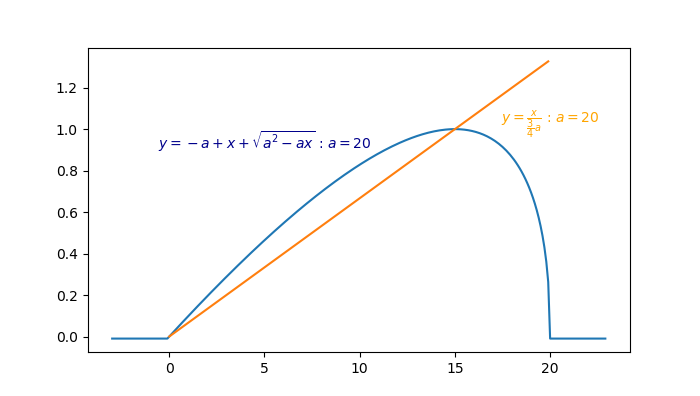
\includegraphics[width=0.7\linewidth]{Figures/code/reward-velocity}
	\caption{نمودار تابع محاسبه \ws{reward} سرعت نرمال شده}
	\label{fig:reward-velocity}
\end{figure}


نمودار این تابع در \ref{fig:reward-velocity} آمده است که با تابع خطی که از مقدار بیشینه آن عبور می‌کند مقایسه شده است.

\begin{alphabetlist}
	\item 
	تا قبل از مقدار بیشینه مقدار این دو تابع نزدیک یک دیگر می‌باشد و شیب آن‌ها نیز به هم نزدیک است. 
	\item 
	این تابع پس از مقدار رسیدن به مقدار بیشینه خود، به صورت نزولی افت می‌کند.
	\item
	اگر از نقطه‌ای که مقدار بیشینه در آن رخ می‌دهد، به سمت مثبت حرکت کنیم سریع تر از هنگامی‌که به سمت منفی حرکت می‌کند.
	\item 
	دیگر ویژگی آن این است که در حدود مقدار بیشینه خود، تقریبا هموار است که این هموار بودن آن موجب آن خواهد شد که \w{agent} بتواند در حوالی سرعت بیشینه خود بدون تفاوت زیادی در مقدار \w{reward} تصمیم بگیرد که سرعت را در صورت لزوم کم و یا زیاد کند.
\end{alphabetlist}


\begin{remark}[خیلی مهم]
چیزی که به عنوان متغیر مستقل به تابع ارسال می‌شود سرعت است اما با سرعت واقعی متفاوت است. در حقیقت میانگین وزن‌داری از سرعت واقعی و سرعت دستوری می‌باشد. منظور از سرعت دستوری همان سرعتی است که با استفاده از دستورات کنترلی برای محیط شبیه سازی فرستاده می‌شود.
\[
V = 0.8 V_{\mathrm{sim}} + 0.2 V_{\mathrm{cmd}}
\]
\end{remark}

علت این تفاوت نیز به سیاست‌های تشویقی مربوط می‌شود. فرض کنید \w{agent} تصمیم می‌گیرد سرعت را افزایش دهد. با این تصمیم مقدار سرعت 5 واحد افزایش می‌یابد. ولی سرعت بعد از گذشت از یک \w{step} به مقدار کمی سرعت آن افزایش یافته است از این رو \w{reward} کمی می‌گیرد. با این میانگین‌گیری در حقیقت برای تصمیم و نیت خوب \w{agent} مقداری \w{reward} در نظر گرفته ‌می‌شود تا مقدار \w{reward} بیشتری را بگیرد. 

درصورتی که \w{agent} 
تصمیم بگیرد که سرعت خود را کم کند، بابت این تصمیم که نامطلوب است جریمه می‌شود. مقدار این جریمه کمتر از مقدار تشویق است. این موضوع در نزدیکی های سرعت بیشینه کمک کننده خواهد بود. زیرا بالا بردن سرعت در آن حوالی مطلوب نیست بنابراین در صورتی که نیت کند که سرعت زیاد شود، این تصمیم \w{agent} همراه با افت \w{reward} بیشتری (نسبت به حالتی که نیت در نظر گرفته نشده است) خواهد بود. بنابراین این تفاوت ها مطلوب و سازنده خواهد بود. 

آخرین \w{reward}، $\mathcal{R}_{\mathrm{Nearby}}$ می‌باشد. بخاطر مشکلات شبیه‌سازی در اثر تغییر لاین، این تغییر به تمامی اعمال نمی‌شود و ممکن است \w{agent} در فاصله بسیار نزدیک از یک ماشین دیگر رانندگی کند به گونه‌ای که تصادف رخ ندهد. هدف از ایجاد این \w{reward} نیز ایجاد یک حس خطر است. مسلماً باید علامت آن منفی باشد. 

برای این منظور به نوعی دو سنسور مجازی در کناره های \w{agent} کار گذاشته شد.
درصورتی که ماشین دیگر در فاصله $1.5$متری از \w{agent} در جهت های داده شده در شکل \ref{subfig:agent-nearby-reward} قرار داشته‌باشد، مقدار آن صفر ‌خواهد بود و در صورتی که فاصله از این مقدار کمتر شود به صورت خطی تا $-2.5$ \w{reward} منفی دریافت می‌کند.

نمودار تابع در شکل \ref{subfig:agent-nearby-reward} آمده است و ضابطه آن به صورت زیر می‌باشد:
\[
\left.F^{\mathcal{R}_{\mathrm{Nearby}}}\right|_{R,W} = \left\{
\begin{array}{lcc}
-\dfrac{R}{W} x + R &:& x \in [0,W] \\
0 &:& \text{\rl{سایر نقاط}}
\end{array}
\right.
\]

که در رابطه فوق، مقدار $W$ طول سنسور مجازی و اندازه $R$ بیش‌ترین امتیاز (اما در جهت منفی) که در این نمودار اتفاق می‌افتد.



\begin{figure}
%	\def\localheight{5cm}
	\centering
	\subfigure[تابع \ws{reward} در زمان نزدیکی]{
		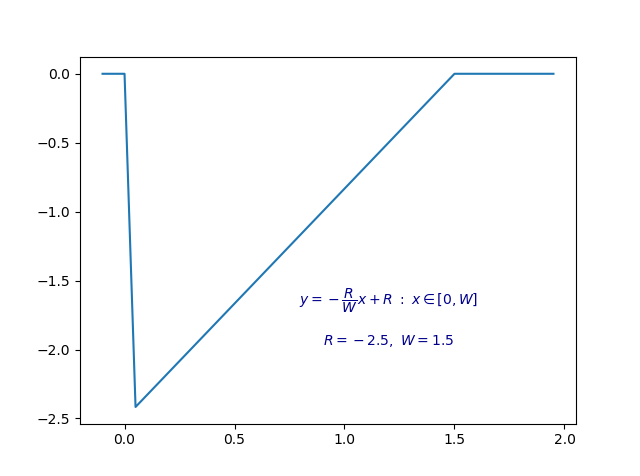
\includegraphics[height=5cm]{Figures/code/nearby-reward}
		\label{subfig:nearby-reward}
	}
	\subfigure[محل قرار گیری سنسور‌های مجازی بر روی \ws{agent}]{
		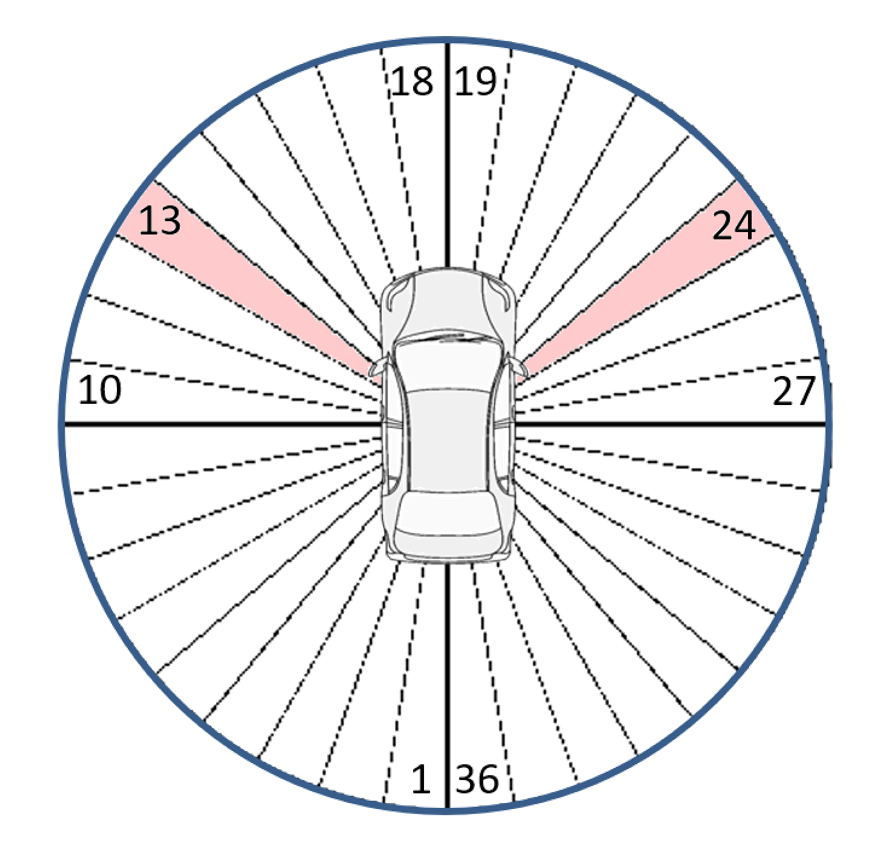
\includegraphics[height=5cm]{Figures/rzbinary/agent-nearby-reward}
		\label{subfig:agent-nearby-reward}
	}
\caption{تابع \ws{reward} نزدیکی و محل قرار گیری این تابع در فضای \w{obs}}
\label{fig:agent-nearby}
\end{figure}



\subsection{بررسی مقدار $\gamma$}

مقدار $\gamma$ در لایه الگوریتم مطرح می‌شود. در الگوریتم \gls{a:dqn} این پارامتر، مقدار دید روبه جلو را نشان ‌می‌دهد.








